В данном разделе приводятся численные результаты, полученные с помощью реализованного метода оконного ДП, и описывается независимая верификация методом Monte-Carlo. Все упоминаемые исполняемые файлы (\texttt{windowed\_dp\_universal}, \texttt{monte\_carlo\_universal}) собираются из исходников открытого git-репозитория работы~\cite{ourgithub} согласно командам компиляции из приложения~Б.

\subsection{Постановка экспериментов}

\textbf{Оборудование.} Эксперименты выполнялись на двух машинах:
\begin{itemize}
    \item \emph{Локальная} --- ноутбук Apple~MacBook с процессором Apple~M-серии (\texttt{arm64}, 8 ядер, 3{,}2~ГГц), 16~ГБ оперативной памяти, macOS~14. Компилятор: \texttt{clang++/g++} с опциями \texttt{-O3 -ffast-math -std=c++17 -funroll-loops}. Векторные расширения NEON используются по умолчанию.
    \item \emph{Серверная} --- x86\_64 узел (Intel Xeon класса Cascade Lake, 16~ядер, 2{,}1~ГГц), $\geq 64$~ГБ оперативной памяти, Linux. Компилятор: \texttt{g++~11.4} с опциями \texttt{-O3 -ffast-math -std=c++17 -funroll-loops -mavx2 -mbmi -mbmi2}. Длительные запуски ($N \geq 11$) выполнялись здесь.
\end{itemize}
Все запуски --- однопоточные на одном физическом ядре.

\textbf{Бинарный алфавит ($\sigma = 2$).} Параметры $(N, \mathrm{MAX\_SH}, K)$ подбирались итеративно: при фиксированных $\mathrm{MAX\_SH}$ и $K$ увеличивался $N$ до достижения предела памяти; затем при фиксированном $N$ варьировались $\mathrm{MAX\_SH}$ и $K$.

\textbf{Алфавиты $\sigma = 3, \ldots, 10$.} Для каждого $\sigma$ параметры подбирались с учётом ограничения $\mathrm{MASK\_BITS} = N \lceil \log_2 \sigma \rceil \leq 24$. При больших $\sigma$ выгодны малые $N = 3$ и относительно большие $\mathrm{MAX\_SH}$.

\subsection{Главный результат: $\gamma_2 \geq 0{,}7964$}

Рекордный запуск версии x6:
\begin{itemize}
    \item параметры: $N = 12$, $\mathrm{MAX\_SH} = 30$, $K = 40\,000$;
    \item время счёта: $\approx 5$~часов на одном ядре;
    \item память: $\approx 2$~ГБ;
    \item полученная нижняя оценка: $\gamma_2 \geq 0{,}79644$ (округлённо $\gamma_2 \geq 0{,}7964$).
\end{itemize}
Контрольный пересчёт на меньших параметрах в типе \texttt{double} даёт совпадение в первых $5$--$6$ значащих знаках, что подтверждает корректность float-арифметики.

\subsection{Результаты для $\sigma = 3, \ldots, 10$}

В таблице~\ref{tab:large-sigma} приведены полученные оценки для $\sigma \in \{3, \ldots, 10\}$ в сравнении с лучшим опубликованным результатом~\cite{heineman2024}.

\begin{table}[h!]
\caption{Нижние оценки $\gamma_\sigma$ для $\sigma = 3, \ldots, 10$}
\label{tab:large-sigma}
\centering
\small
\begin{tabular}{|c|l|c|c|c|}
\hline
$\sigma$ & Параметры $(N, \mathrm{SH}, K)$ & Наш $\gamma_\sigma \geq$ & Heineman'24~\cite{heineman2024} & Прирост \\
\hline
3   & $(5, 25, 3\,200)$  & $0{,}6834$ & $0{,}6822$ & $+0{,}17\,\%$ \\
4   & $(6, 30, 3\,000)$\footnote{Получен в коммите \texttt{2f726f0} (``alphabet4 new record'') git-репозитория~\cite{ourgithub}; параметры см.\ в приложении~Г.} & $0{,}6230$ & $0{,}6143$ & $+1{,}42\,\%$ \\
5   & $(3, 35, 4\,500)$  & $0{,}5576$ & $0{,}5498$ & $+1{,}42\,\%$ \\
6   & $(3, 35, 3\,500)$  & $0{,}5198$ & $0{,}4992$ & $+4{,}12\,\%$ \\
7   & $(3, 45, 4\,000)$  & $0{,}4893$ & $0{,}4665$ & $+4{,}89\,\%$ \\
8   & $(3, 27, 2\,700)$  & $0{,}4626$ & $0{,}4388$ & $+5{,}42\,\%$ \\
9   & $(3, 17, 1\,150)$  & $0{,}4363$ & $0{,}4149$ & $+5{,}17\,\%$ \\
10  & $(3, 13, 720)$     & $0{,}4132$ & $0{,}3938$ & $+4{,}93\,\%$ \\
\hline
\end{tabular}
\end{table}

Прирост к существующему рекорду растёт с увеличением $\sigma$: для малых $\sigma$ метод~\cite{heineman2024} использует расширенные пространства состояний, для больших --- упирается в комбинаторный взрыв, тогда как параметризация $(N, \mathrm{MAX\_SH})$ настоящего метода позволяет адаптироваться.

\subsection{Зависимость от параметров метода}

На рис.~\ref{fig:vs-N} показана зависимость $\gamma_{2, N, 30}$ от $N \in \{7, 8, \ldots, 12\}$ при фиксированном $\mathrm{MAX\_SH} = 30$: значение монотонно растёт с увеличением $N$ и проявляет признаки насыщения. Полная таблица данных приведена в приложении~Г (таблица~\ref{tab:N-dep-appendix}).

\begin{figure}[h!]
\centering
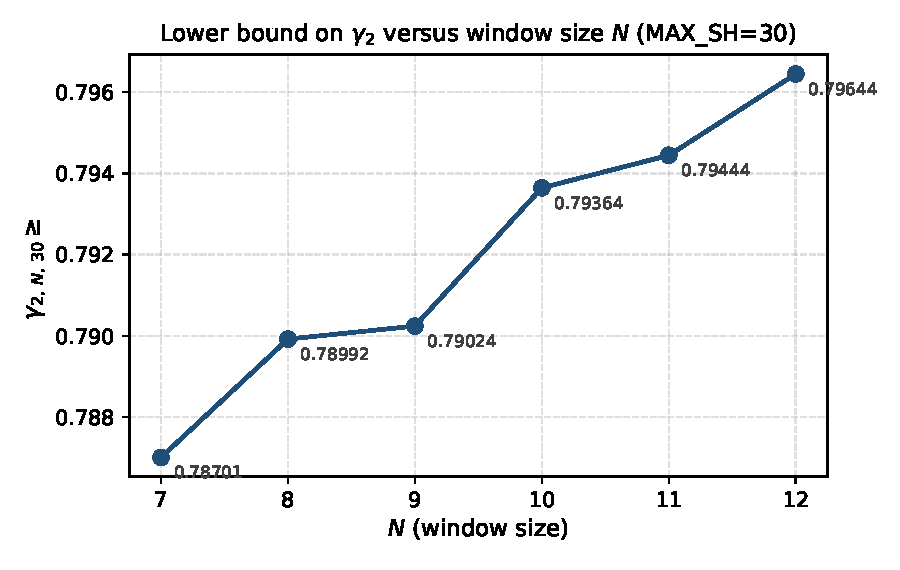
\includegraphics[width=0.78\textwidth]{figures/gamma2_vs_N.pdf}
\caption{Зависимость нижней оценки $\gamma_{2, N, 30}$ от размера окна $N$. Данные из приложения~Г.}
\label{fig:vs-N}
\end{figure}

Аналогично, при фиксированном $N$ значение $\gamma_{2, N, \mathrm{MAX\_SH}}$ растёт с увеличением $\mathrm{MAX\_SH}$ и насыщается; зависимость от $K$ выходит на плато после нескольких тысяч итераций.

На рис.~\ref{fig:vs-sigma} показаны полученные нижние оценки $\gamma_\sigma$ для $\sigma = 2, \ldots, 10$ в сравнении с эмпирическими средними Monte-Carlo и с результатами~\cite{heineman2024}. Все три кривые монотонно убывают по $\sigma$ в согласии с асимптотикой $\gamma_\sigma \sim 2/\sqrt{\sigma}$.

\begin{figure}[h!]
\centering
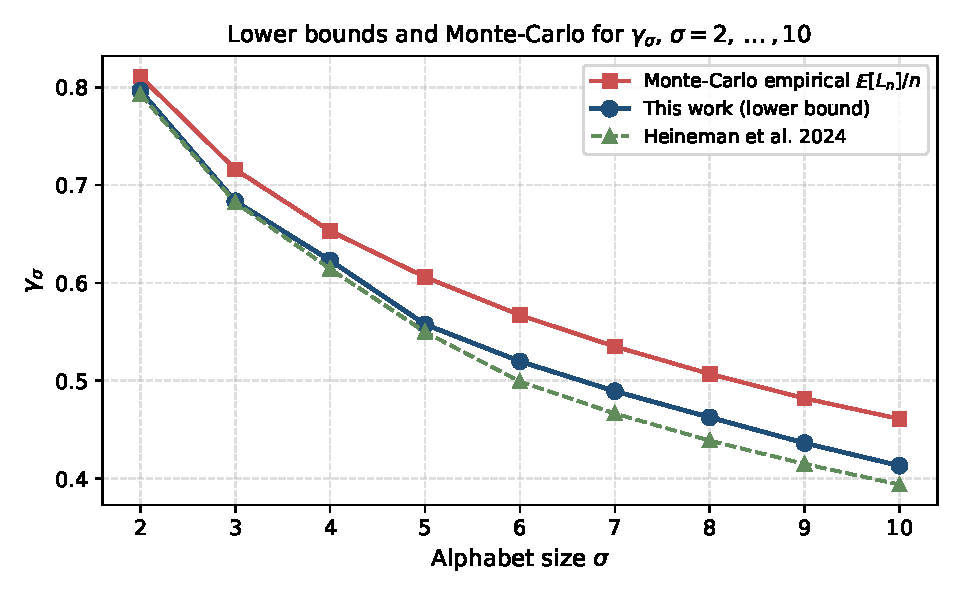
\includegraphics[width=0.86\textwidth]{figures/gamma_vs_sigma.pdf}
\caption{Сравнение нижних оценок $\gamma_\sigma$ (настоящая работа vs.~\cite{heineman2024}) и эмпирического Monte-Carlo среднего для $\sigma = 2, \ldots, 10$.}
\label{fig:vs-sigma}
\end{figure}

\subsection{Верификация Monte-Carlo}

Для каждого $\sigma \in \{2, 3, \ldots, 10\}$ запускалась независимая программа, скомпилированная из файла \texttt{src/monte\_carlo\_universal.cpp} в git-репозитории работы~\cite{ourgithub} и реализующая классический ДП-LCS на парах независимых равномерных строк. Параметры запуска:
\begin{itemize}
    \item длина строк: $n = 10\,000$ (для $\sigma \leq 4$ --- также $n = 20\,000$);
    \item число испытаний: $T = 500$;
    \item начальное состояние генератора: \texttt{seed = 42} для воспроизводимости.
\end{itemize}

\textbf{Обоснование размера выборки.} По эмпирическим оценкам стандартное отклонение случайной величины $L_n/n$ для $n = 10\,000$ составляет $\mathrm{sd}(L_n/n) \approx 0{,}004$ (бинарный алфавит, оценка по предварительным $T = 100$ запускам). Тогда стандартная ошибка эмпирического среднего $\overline{L_n/n}$ по $T = 500$ испытаниям:
\[
    \mathrm{SE} = \mathrm{sd}/\sqrt{T} \approx 0{,}004/\sqrt{500} \approx 1{,}8 \cdot 10^{-4},
\]
а $95\,\%$-доверительный интервал имеет ширину $\pm 2\,\mathrm{SE} \approx \pm 3{,}6 \cdot 10^{-4}$, что заметно меньше характерных зазоров между нашей оценкой и MC-средним ($\geq 0{,}015$). Следовательно, точность MC-проверки достаточна для строгого вывода о непревышении.

\begin{table}[h!]
\caption{Сравнение нижних оценок и Monte-Carlo среднего}
\label{tab:mc}
\centering
\small
\begin{tabular}{|c|c|c|c|c|}
\hline
$\sigma$ & $\mathbb{E}[L_n]/n$ (MC) & Наша $\gamma_\sigma \geq$ & Зазор до MC & Зазор, \% от MC \\
\hline
2  & $\approx 0{,}811$  & $0{,}7964$ & $\approx 0{,}015$ & $\approx 1{,}8\,\%$ \\
3  & $\approx 0{,}716$  & $0{,}6834$ & $\approx 0{,}032$ & $\approx 4{,}5\,\%$ \\
4  & $\approx 0{,}653$  & $0{,}6230$ & $\approx 0{,}030$ & $\approx 4{,}6\,\%$ \\
5  & $\approx 0{,}606$  & $0{,}5576$ & $\approx 0{,}048$ & $\approx 7{,}9\,\%$ \\
6  & $\approx 0{,}567$  & $0{,}5198$ & $\approx 0{,}047$ & $\approx 8{,}3\,\%$ \\
7  & $\approx 0{,}535$  & $0{,}4893$ & $\approx 0{,}046$ & $\approx 8{,}6\,\%$ \\
8  & $\approx 0{,}507$  & $0{,}4626$ & $\approx 0{,}044$ & $\approx 8{,}7\,\%$ \\
9  & $\approx 0{,}482$  & $0{,}4363$ & $\approx 0{,}046$ & $\approx 9{,}5\,\%$ \\
10 & $\approx 0{,}461$  & $0{,}4132$ & $\approx 0{,}048$ & $\approx 10{,}4\,\%$ \\
\hline
\end{tabular}
\end{table}

Все нижние оценки строго не превосходят соответствующих эмпирических средних, что является необходимым условием корректности метода. Зазор $\approx 0{,}015$ для $\sigma = 2$ сокращается по сравнению с зазором $\approx 0{,}018$ для предыдущей лучшей нижней оценки $0{,}7927$.

\subsection{Сравнение с историей задачи}

Прирост настоящей работы к лучшей опубликованной нижней оценке $\gamma_2$ составил $0{,}7964 - 0{,}7927 \approx +0{,}0037$. Для сравнения:
\begin{itemize}
    \item за 1975--2003 (28 лет): прирост $0{,}7881 - 0{,}7615 = +0{,}0266$;
    \item за 2003--2024 (21 год): прирост $0{,}79266 - 0{,}7881 \approx +0{,}0046$;
    \item настоящая работа: $+0{,}0037$ за один шаг.
\end{itemize}
Таким образом, метод оконного ДП дал прирост, сравнимый с суммарным прогрессом задачи за 21~год.

\emph{Замечание.} Прямое сравнение «один шаг vs.~годы» условно: исторические улучшения опирались на принципиально различные подходы (расширенные конечные автоматы, MCMC-методы, барьерные конструкции), а величина прироста не является монотонно сравнимой характеристикой работ. Тем не менее, абсолютный размер прироста $+0{,}0037$ сравним с суммарным прогрессом 2003--2024~гг., что является объективным фактом.

\subsection*{Выводы по разделу}
\addcontentsline{toc}{subsection}{Выводы по разделу 5}

\begin{enumerate}
    \item Получена рекордная нижняя оценка $\gamma_2 \geq 0{,}7964$ при параметрах $N = 12$, $\mathrm{MAX\_SH} = 30$, $K = 40\,000$.
    \item Получены рекордные нижние оценки $\gamma_\sigma$ для всех $\sigma \in \{3, \ldots, 10\}$ с приростом до $+5{,}42\,\%$ относительно~\cite{heineman2024}.
    \item Все оценки независимо верифицированы Monte-Carlo: ни одна не превосходит эмпирического среднего.
    \item Прирост $+0{,}0037$ для $\gamma_2$ сопоставим с суммарным прогрессом задачи за 2003--2024 годы.
\end{enumerate}
